\documentclass[pdflatex,compress,mathserif]{beamer}

%\usetheme[dark,framenumber,totalframenumber]{ElektroITK}
\usetheme[darktitle,framenumber,totalframenumber]{ElektroITK}

\usepackage[utf8]{inputenc}
\usepackage[T1]{fontenc}
\usepackage{lmodern}
\usepackage[bahasai]{babel}
\usepackage{amsmath}
\usepackage{amsfonts}
\usepackage{amssymb}
\usepackage{graphicx}
\usepackage{multicol}
\usepackage{lipsum}

\newcommand*{\Scale}[2][4]{\scalebox{#1}{$#2$}}%

\title{PEMODELAN JARINGAN KOMUNIKASI}
\subtitle{The Life of a Packet}

\author{Tim Dosen Pengampu}

\begin{document}

\maketitle

\section{DNS - The Domain Name System}

\begin{frame}
	\frametitle{OSI Reference Model - Encapsulation}
	\begin{center}
		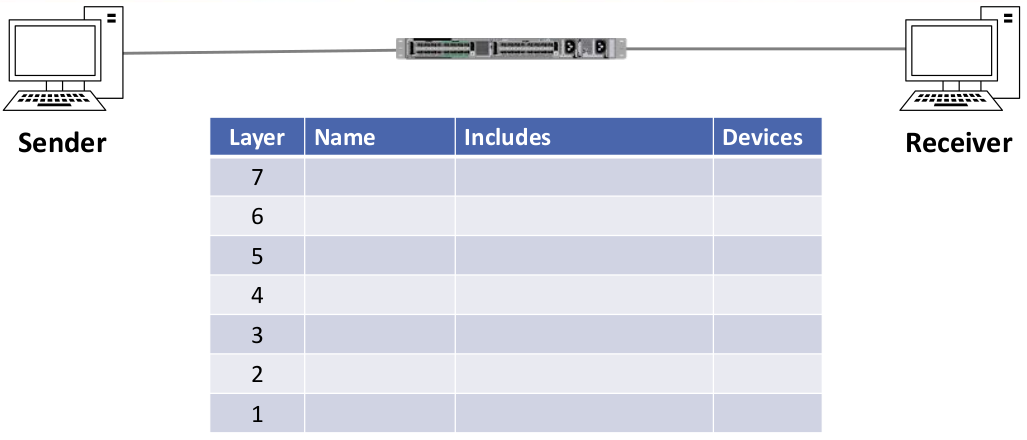
\includegraphics[width=\linewidth]{img/img01}
	\end{center}
\end{frame}

\begin{frame}{OSI Reference Model - Encapsulation}
	\begin{center}
		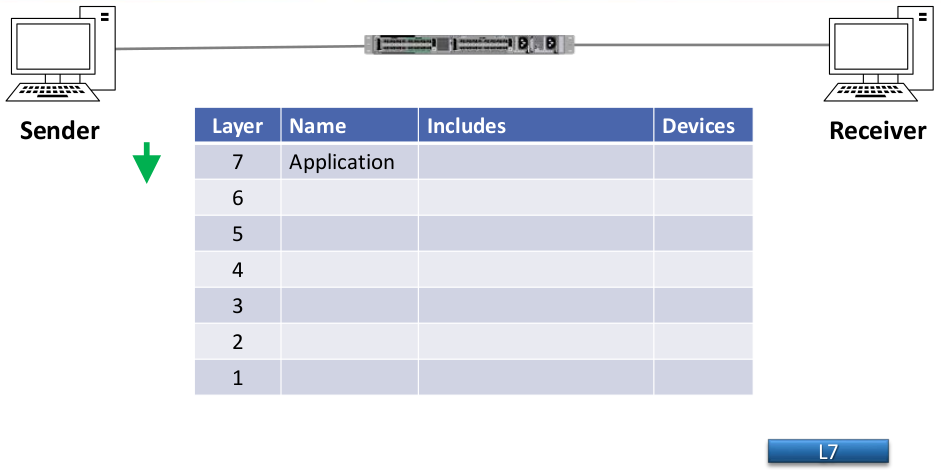
\includegraphics[width=\linewidth]{img/img02}
	\end{center}
\end{frame}

\begin{frame}{OSI Reference Model - Encapsulation}
	\begin{center}
		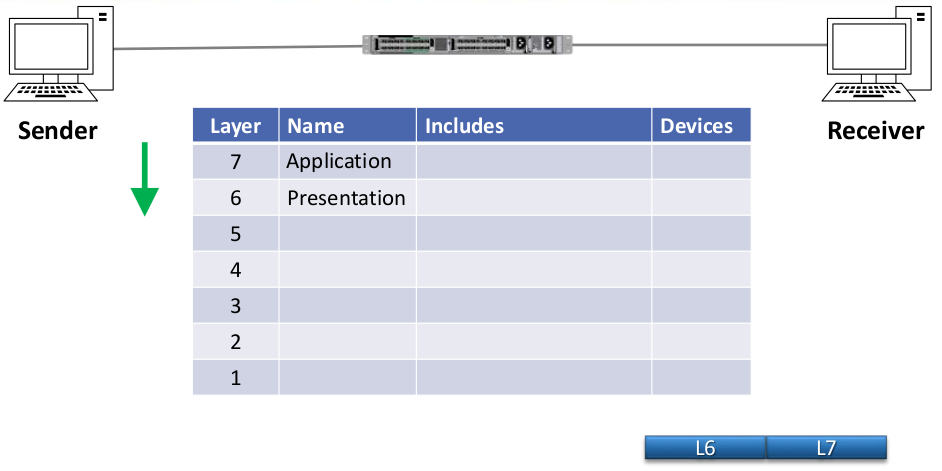
\includegraphics[width=\linewidth]{img/img03}
	\end{center}
\end{frame}

\begin{frame}{OSI Reference Model - Encapsulation}
	\begin{center}
		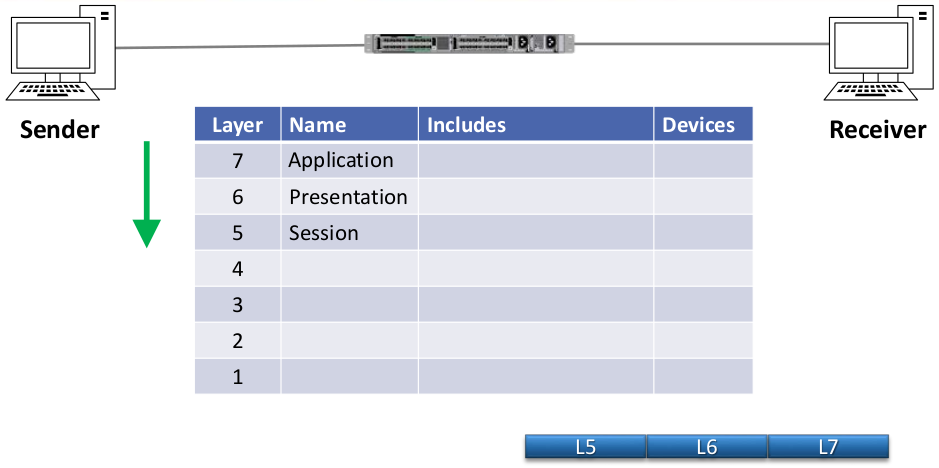
\includegraphics[width=\linewidth]{img/img04}
	\end{center}
\end{frame}

\begin{frame}{OSI Reference Model - Encapsulation}
	\begin{center}
		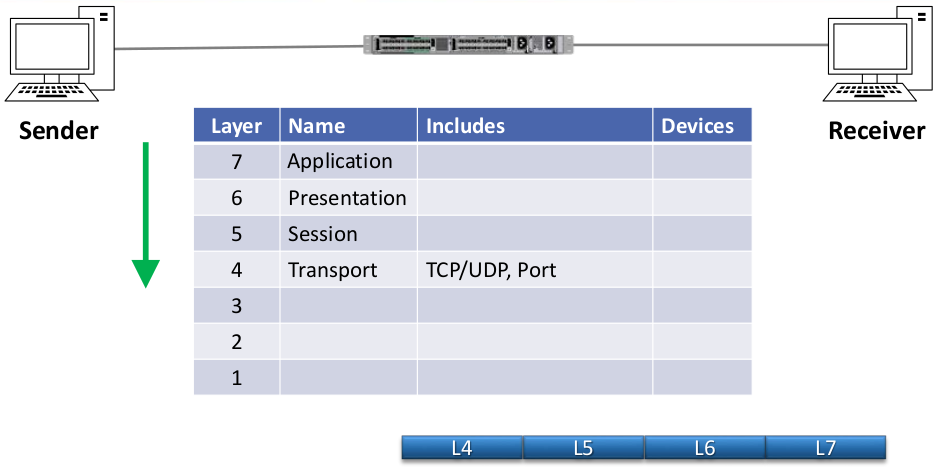
\includegraphics[width=\linewidth]{img/img05}
	\end{center}
\end{frame}

\begin{frame}{OSI Reference Model - Encapsulation}
	\begin{center}
		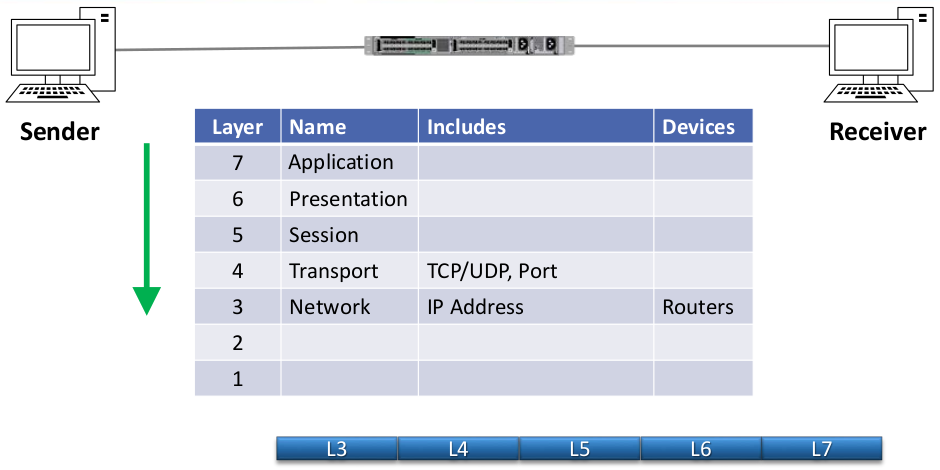
\includegraphics[width=\linewidth]{img/img06}
	\end{center}
\end{frame}

\begin{frame}
	\frametitle{The Domain Name System}
	\begin{itemize}
		\item The Domain Name System (DNS) resolves a Fully Qualified Domain Name (FQDN) such as www.cisco.com to an IP address.
		\item Enterprises will typically have an internal DNS server which can resolve the IP addresses of internal hosts.
		\item Hosts will send their DNS queries to this server.
		\item If the internal DNS server cannot resolve a query, it will forward the request out to public DNS servers on the Internet.
		\item DNS requests are sent using UDP port 53 (and can fail over to TCP).
	\end{itemize}
\end{frame}

\section{DNS on Cisco Routers}

\begin{frame}
	\frametitle{Router DNS Commands}
	\begin{itemize}
		\item DNS Client:
		\begin{itemize}
			\item[] \texttt{ip domain-lookup}
			\item[] \texttt{ip name-server 172.23.4.1}
			\item[] \texttt{ip domain-name flackboxA.lab} (primary domain name)
			\item[] \texttt{ip domain-list flackboxB.lab} (additional DNS suffixes to search)
		\end{itemize}
		\item Additional DNS Server Commands:
		\begin{itemize}
			\item[] \texttt{ip dns server}
			\item[] \texttt{ip host LinuxA 172.23.4.2}
		\end{itemize}
	\end{itemize}
\end{frame}

\section{ARP - Address Resolution Protocol}

\begin{frame}
	\frametitle{OSI Reference Model - Encapsulation}
	\begin{center}
		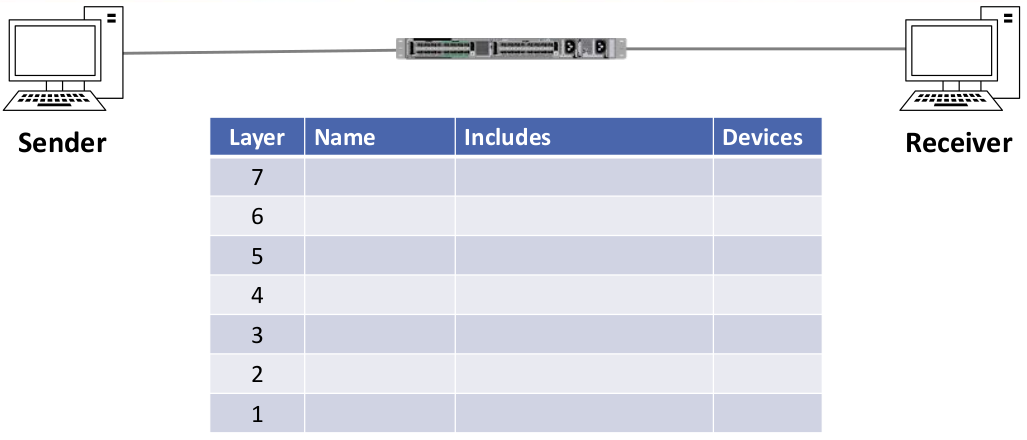
\includegraphics[width=\linewidth]{img/img01}
	\end{center}
\end{frame}

\begin{frame}{OSI Reference Model - Encapsulation}
	\begin{center}
		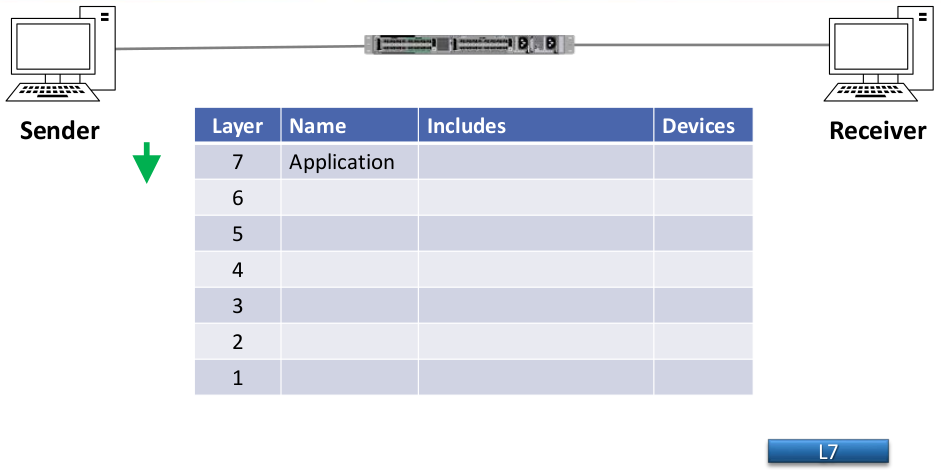
\includegraphics[width=\linewidth]{img/img02}
	\end{center}
\end{frame}

\begin{frame}{OSI Reference Model - Encapsulation}
	\begin{center}
		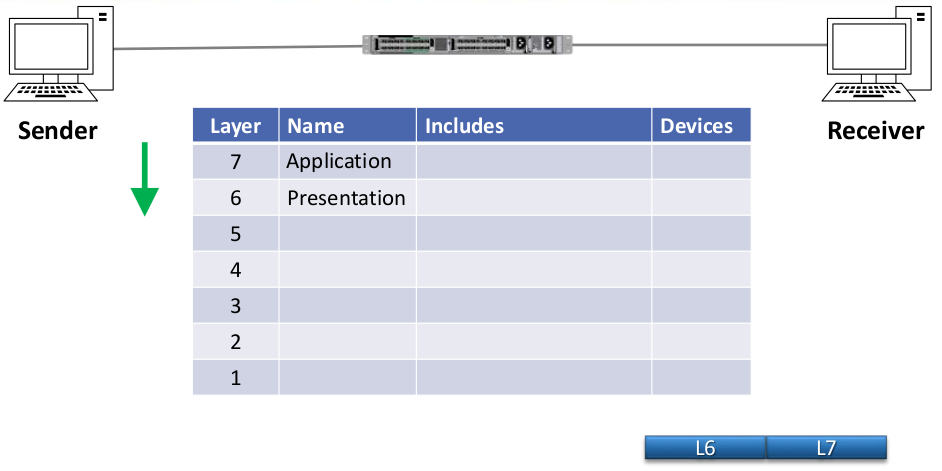
\includegraphics[width=\linewidth]{img/img03}
	\end{center}
\end{frame}

\begin{frame}{OSI Reference Model - Encapsulation}
	\begin{center}
		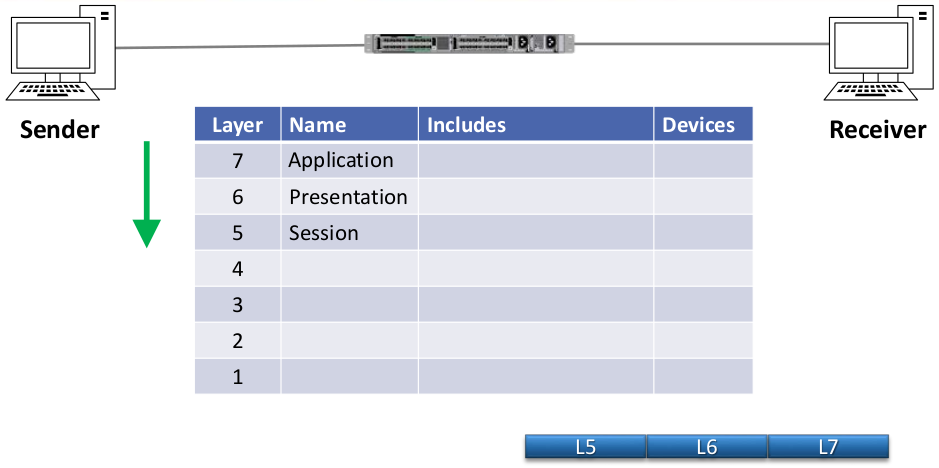
\includegraphics[width=\linewidth]{img/img04}
	\end{center}
\end{frame}

\begin{frame}{OSI Reference Model - Encapsulation}
	\begin{center}
		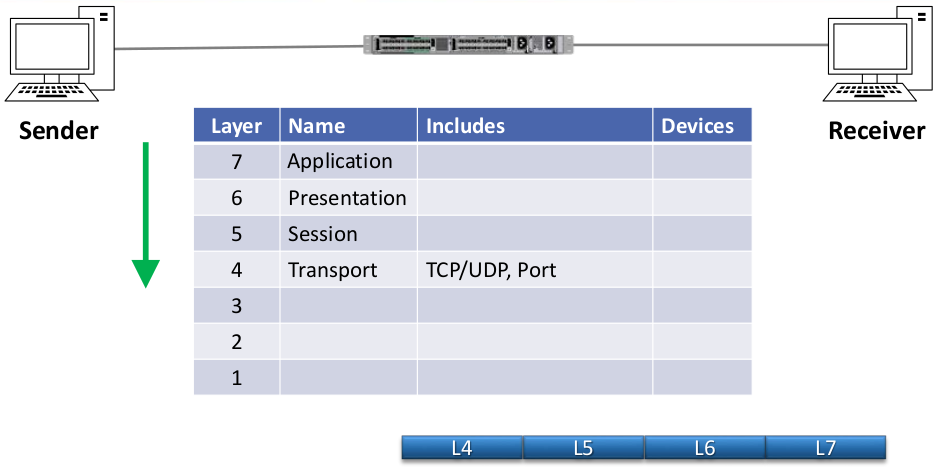
\includegraphics[width=\linewidth]{img/img05}
	\end{center}
\end{frame}

\begin{frame}{OSI Reference Model - Encapsulation}
	\begin{center}
		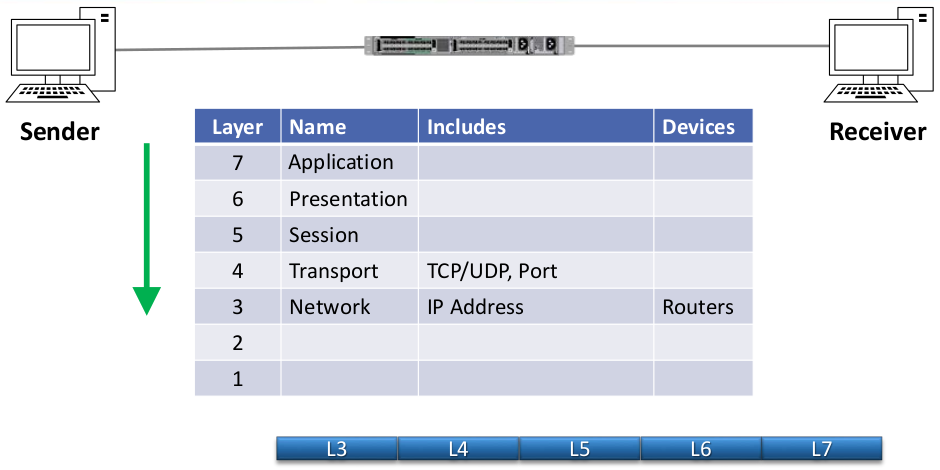
\includegraphics[width=\linewidth]{img/img06}
	\end{center}
\end{frame}

\begin{frame}{OSI Reference Model - Encapsulation}
	\begin{center}
		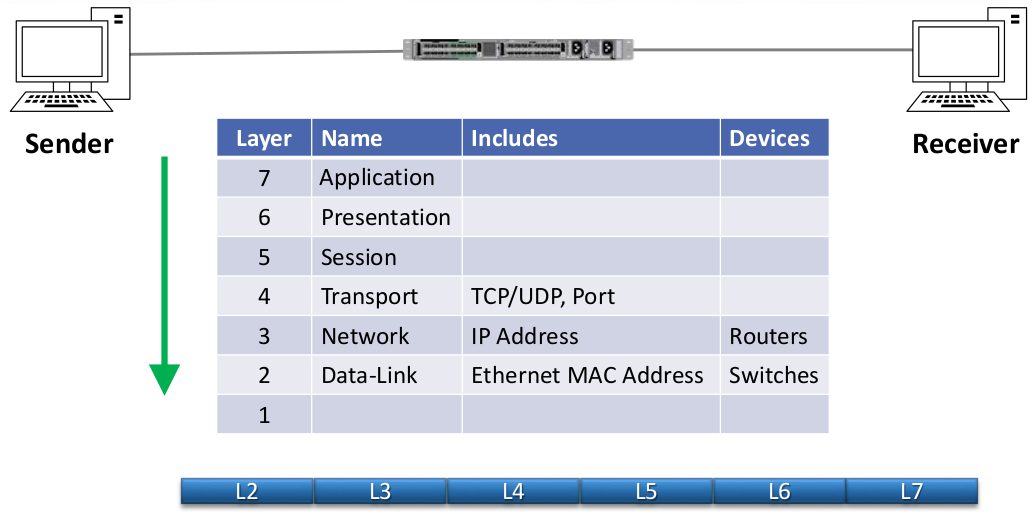
\includegraphics[width=\linewidth]{img/img07}
	\end{center}
\end{frame}

\begin{frame}
	\frametitle{IP to MAC Address Resolution}
	\begin{itemize}
		\item The sender needs to know the receiver’s IP address and MAC address to form the packet it’s going to send
		\item We can point the sender directly at the destination IP address or at a user friendly FQDN such as www.cisco.com
		\item DNS Domain Name System maintains a mapping of FQDNs to IP addresses
		\item ARP Address Resolution Protocol is used to map the IP address to MAC address
	\end{itemize}
\end{frame}

\begin{frame}
	\frametitle{ARP Address Resolution Protocol}
	\begin{center}
		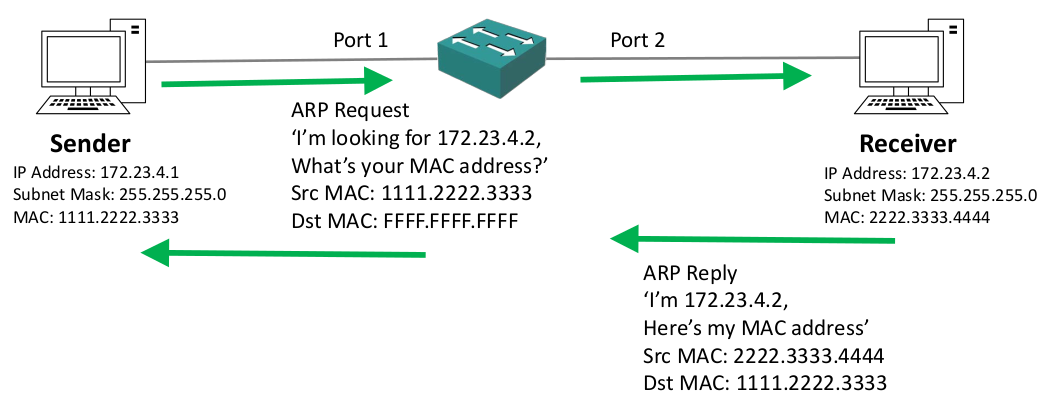
\includegraphics[width=\linewidth]{img/img08}
	\end{center}
\end{frame}

\begin{frame}
	\frametitle{Host ARP Commands}
	\begin{itemize}
		\item ARP replies are saved in a hosts ARP cache so it doesn’t need to send an ARP request every time it wants to communicate
		\item \textbf{Windows}
		\item[] View ARP cache: \texttt{arp -a}
		\item[] Clear ARP cache: \texttt{netsh interface ip delete} arpcache
		\item \textbf{Linux}
		\item[] View ARP cache: \texttt{arp -n}
		\item[] Clear ARP cache: \texttt{ip -s -s neigh flush all}
	\end{itemize}
\end{frame}

\section{ARP for Routed Traffic}

\begin{frame}
	\frametitle{Routed Traffic}
	\begin{itemize}
		\item When the sender and receiver are on different IP subnets, the traffic must be forwarded by a router
		\item In the following example, 172.23.4.1/24 wants to send a packet to 192.168.10.1/24
	\end{itemize}
\end{frame}

\begin{frame}
	\frametitle{Routing Traffic}
	\begin{center}
		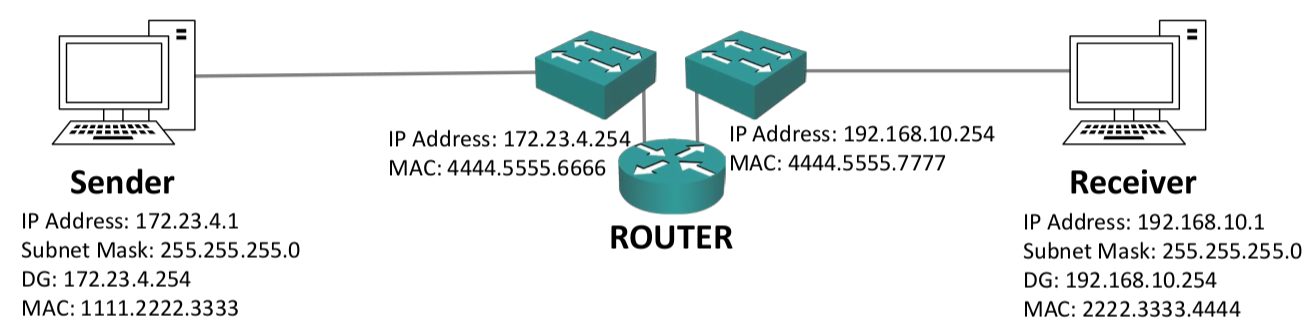
\includegraphics[width=\linewidth]{img/img09}
	\end{center}
\end{frame}

\begin{frame}{Routing Traffic}
	\begin{center}
		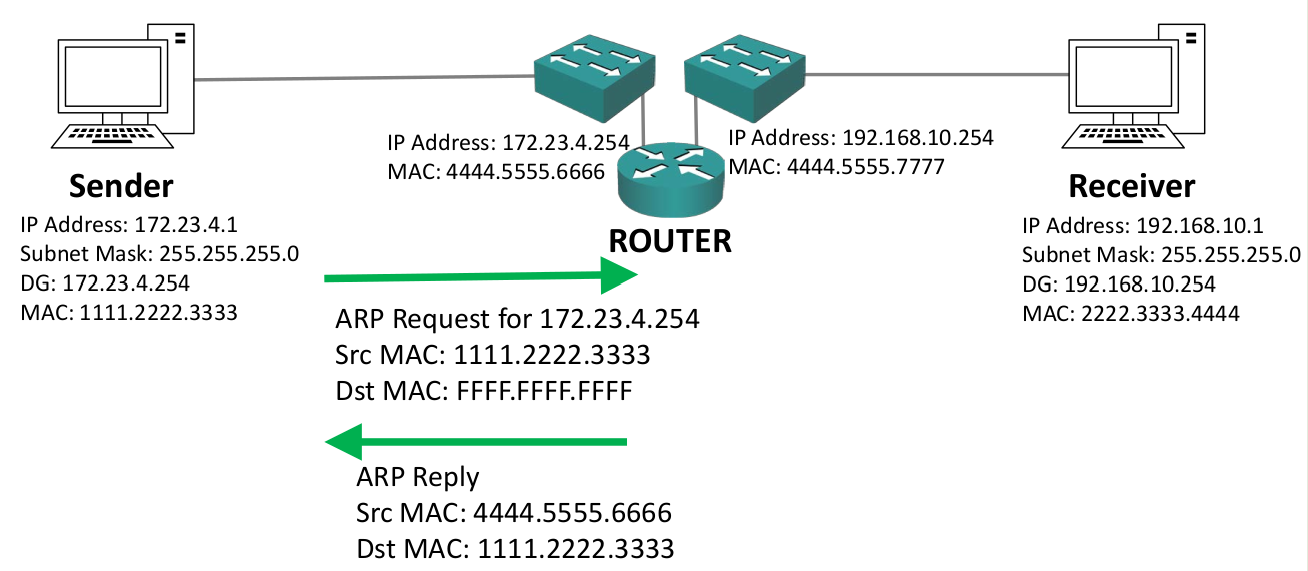
\includegraphics[width=\linewidth]{img/img10}
	\end{center}
\end{frame}

\begin{frame}{Routing Traffic}
	\begin{center}
		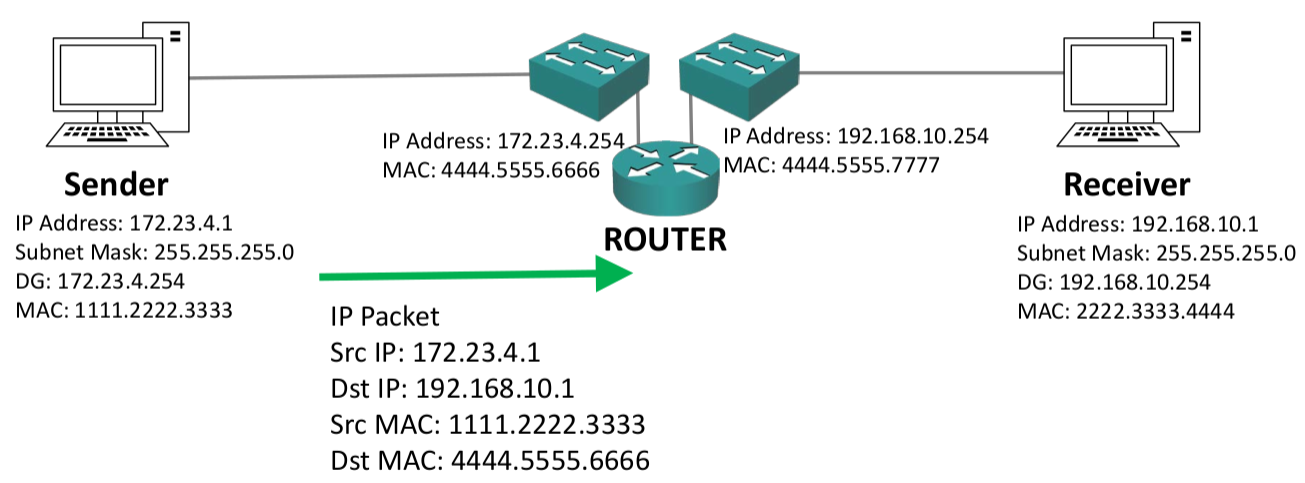
\includegraphics[width=\linewidth]{img/img11}
	\end{center}
\end{frame}

\begin{frame}{Routing Traffic}
	\begin{center}
		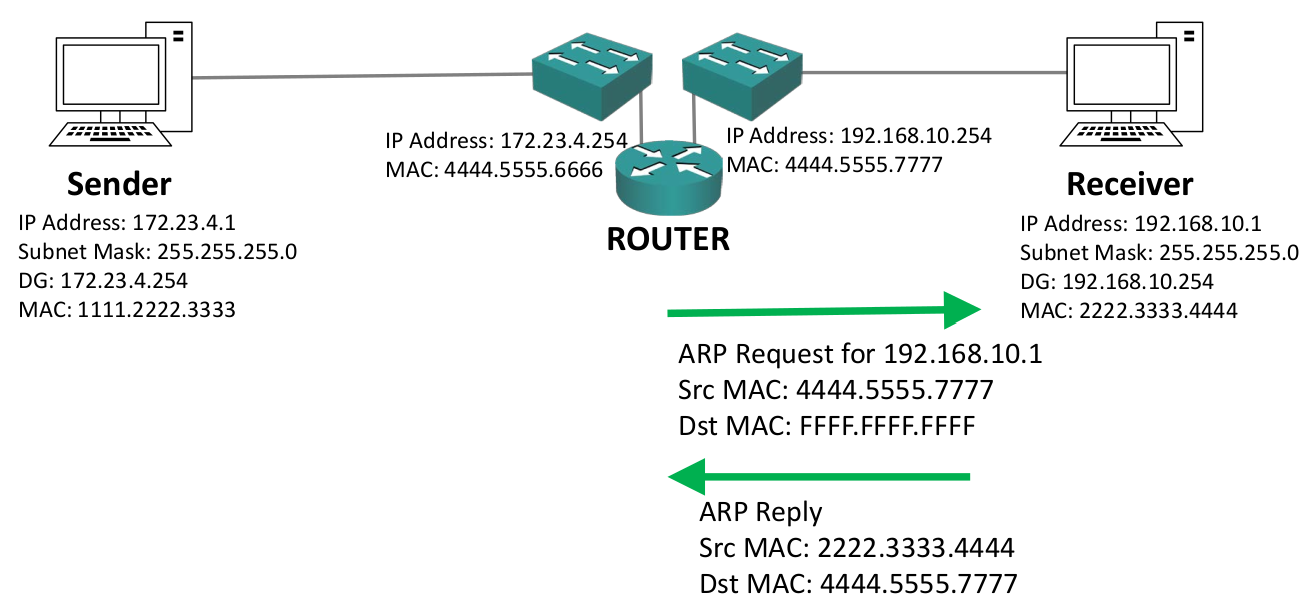
\includegraphics[width=\linewidth]{img/img12}
	\end{center}
\end{frame}

\begin{frame}{Routing Traffic}
	\begin{center}
		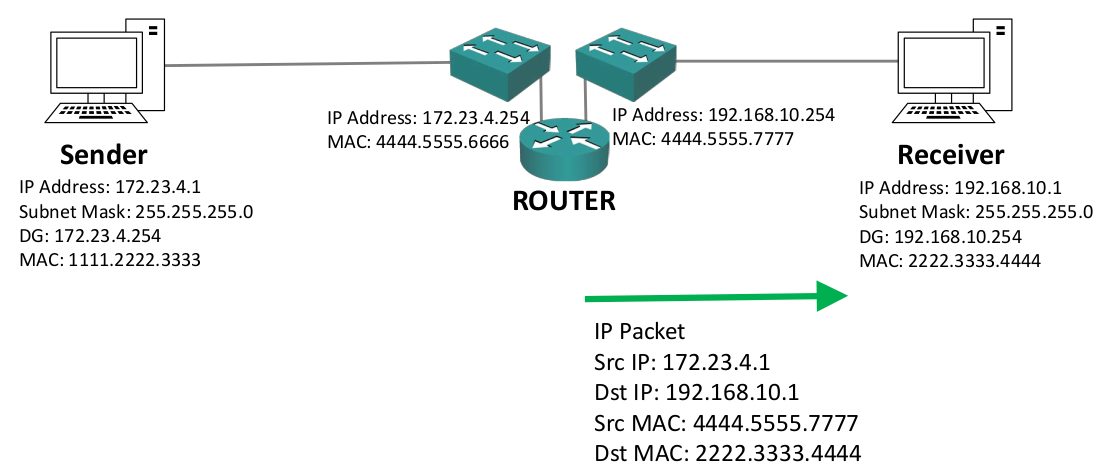
\includegraphics[width=\linewidth]{img/img13}
	\end{center}
\end{frame}

\begin{frame}
	\frametitle{Router ARP Commands}
	\begin{itemize}
		\item View ARP cache: \texttt{show arp}
		\item Clear ARP cache: \texttt{clear arp-cache}
	\end{itemize}
\end{frame}

\section{The Life of a Packet}

\begin{frame}
	\frametitle{The Life of a Packet}
	\begin{center}
		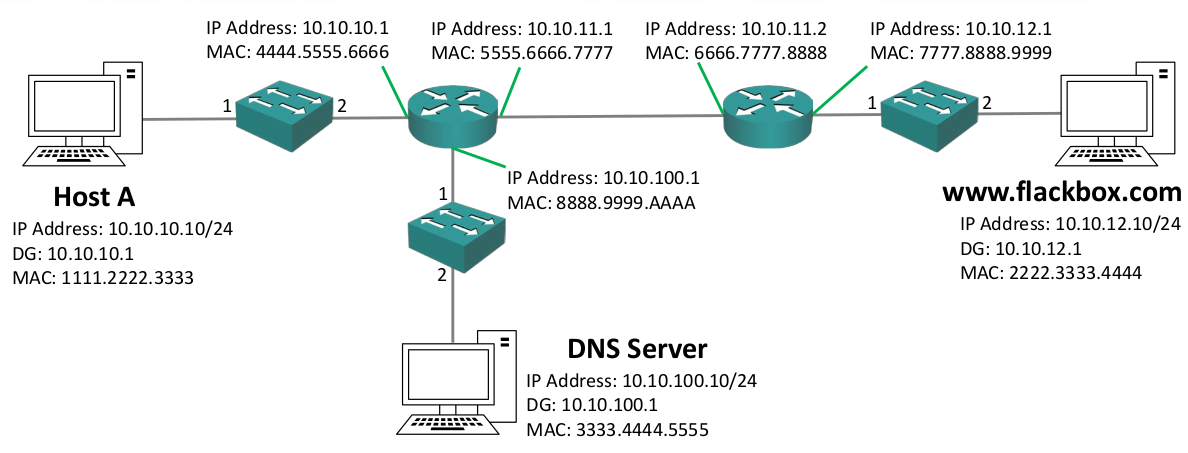
\includegraphics[width=\linewidth]{img/img14}
	\end{center}
\end{frame}

\begin{frame}
	\frametitle{OSI Reference Model - Encapsulation}
	\begin{center}
		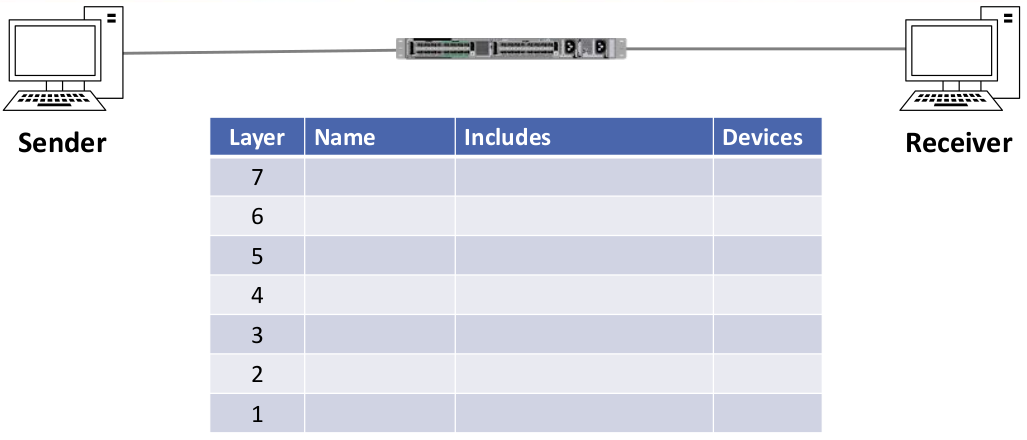
\includegraphics[width=\linewidth]{img/img01}
	\end{center}
\end{frame}

\begin{frame}{OSI Reference Model - Encapsulation}
	\begin{center}
		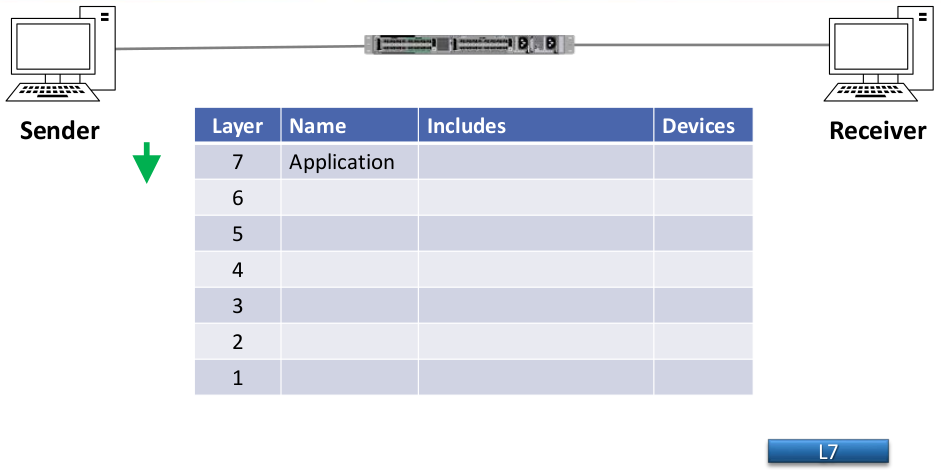
\includegraphics[width=\linewidth]{img/img02}
	\end{center}
\end{frame}

\begin{frame}{OSI Reference Model - Encapsulation}
	\begin{center}
		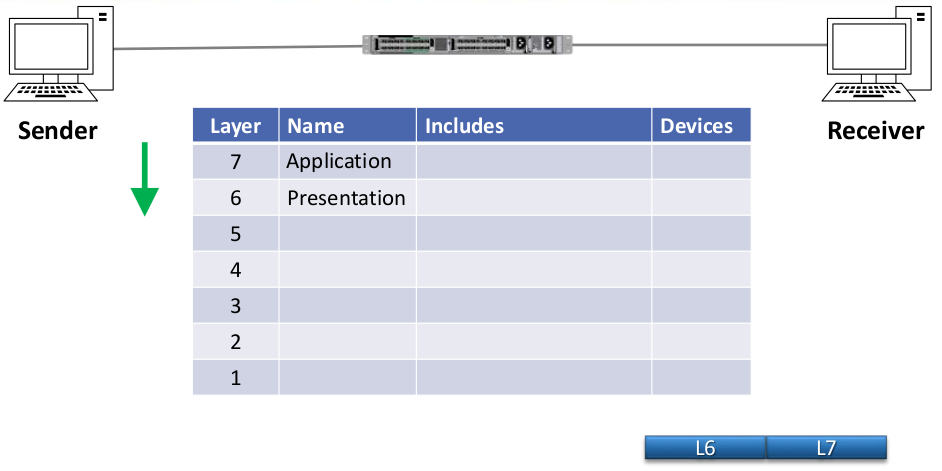
\includegraphics[width=\linewidth]{img/img03}
	\end{center}
\end{frame}

\begin{frame}{OSI Reference Model - Encapsulation}
	\begin{center}
		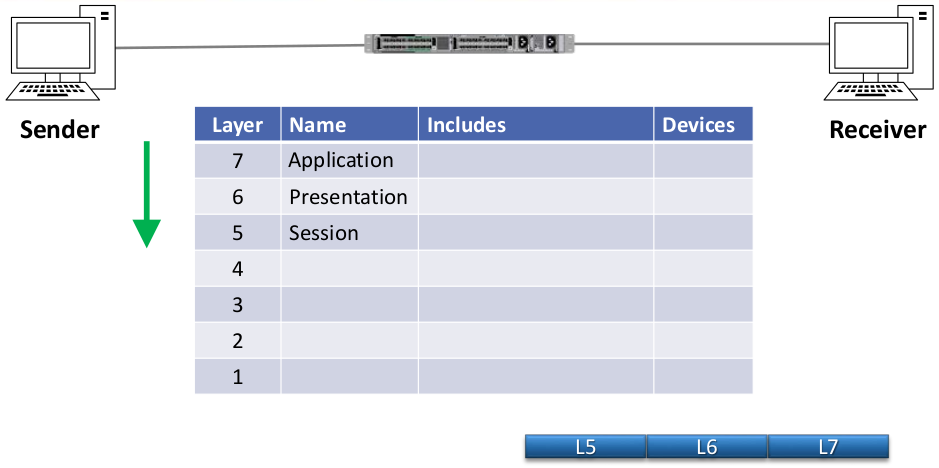
\includegraphics[width=\linewidth]{img/img04}
	\end{center}
\end{frame}

\begin{frame}{OSI Reference Model - Encapsulation}
	\begin{center}
		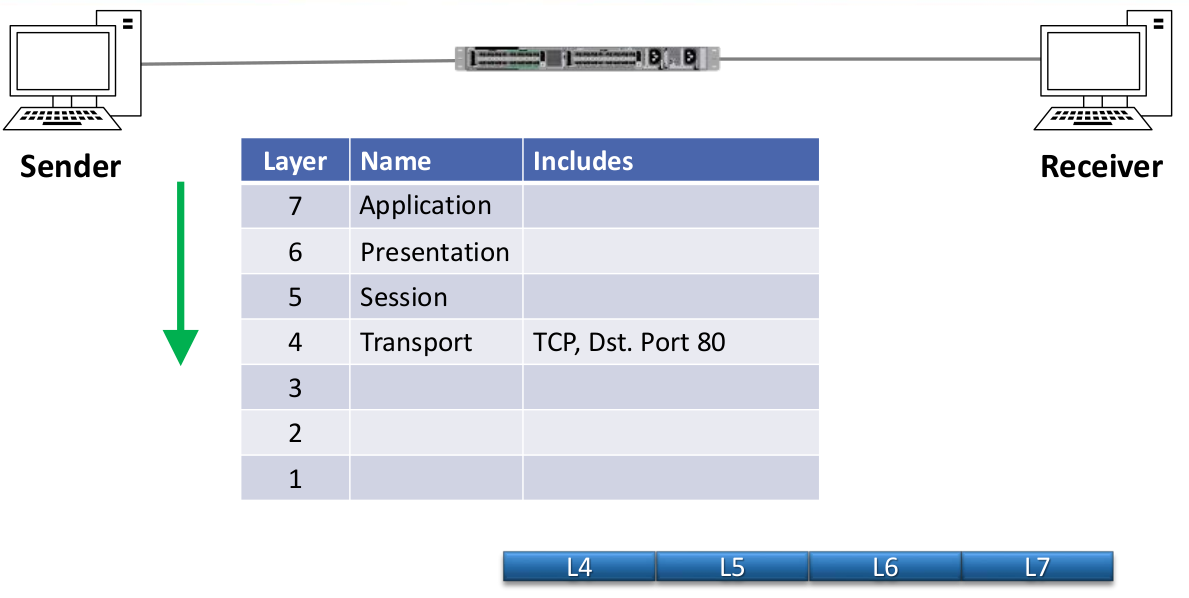
\includegraphics[width=\linewidth]{img/img15}
	\end{center}
\end{frame}


\begin{frame}{OSI Reference Model - Encapsulation}
	\begin{center}
		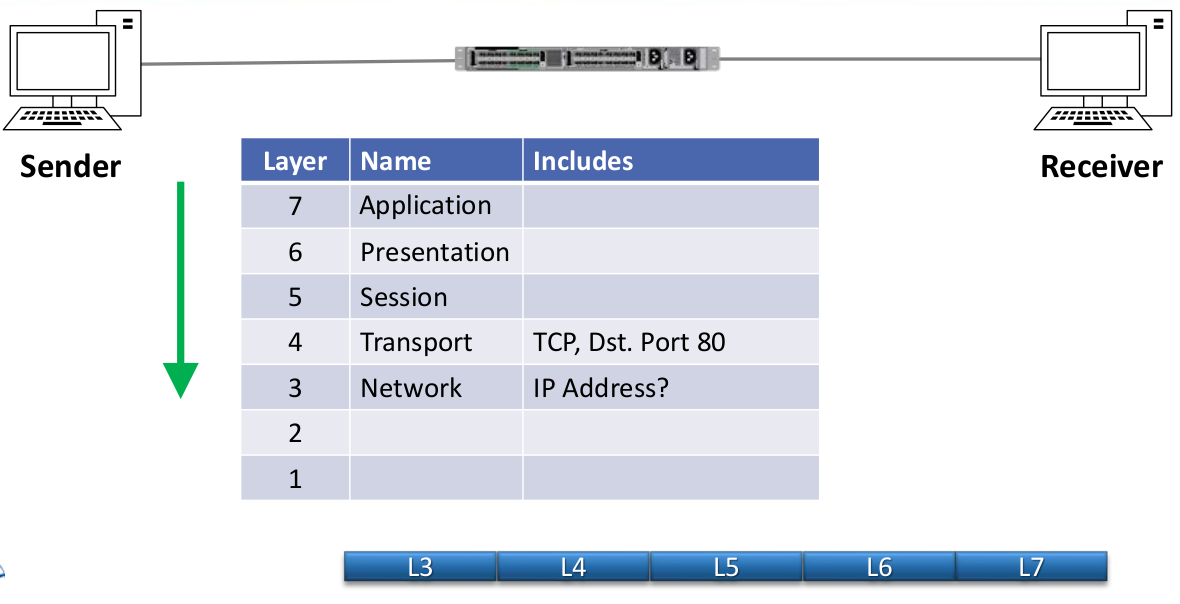
\includegraphics[width=\linewidth]{img/img16}
	\end{center}
\end{frame}

\begin{frame}
	\frametitle{The Life of a Packet}
	\begin{itemize}
		\item Host A (10.10.10.10/24) wants to send a packet to the FQDN www.flackbox.com, but it doesn’t know the destination IP address
		\item It will hold the packet and send a DNS request to its DNS server at 10.10.100.10
		\item Host A compares its IP address and subnet mask to the destination address of the DNS server and sees it is on a different subnet, so the DNS request needs to be sent via its default gateway
		\item Host A will hold the DNS request and send a broadcast ARP request for its default gateway at 10.10.10.1
	\end{itemize}
\end{frame}

\begin{frame}{The Life of a Packet}
	\begin{center}
		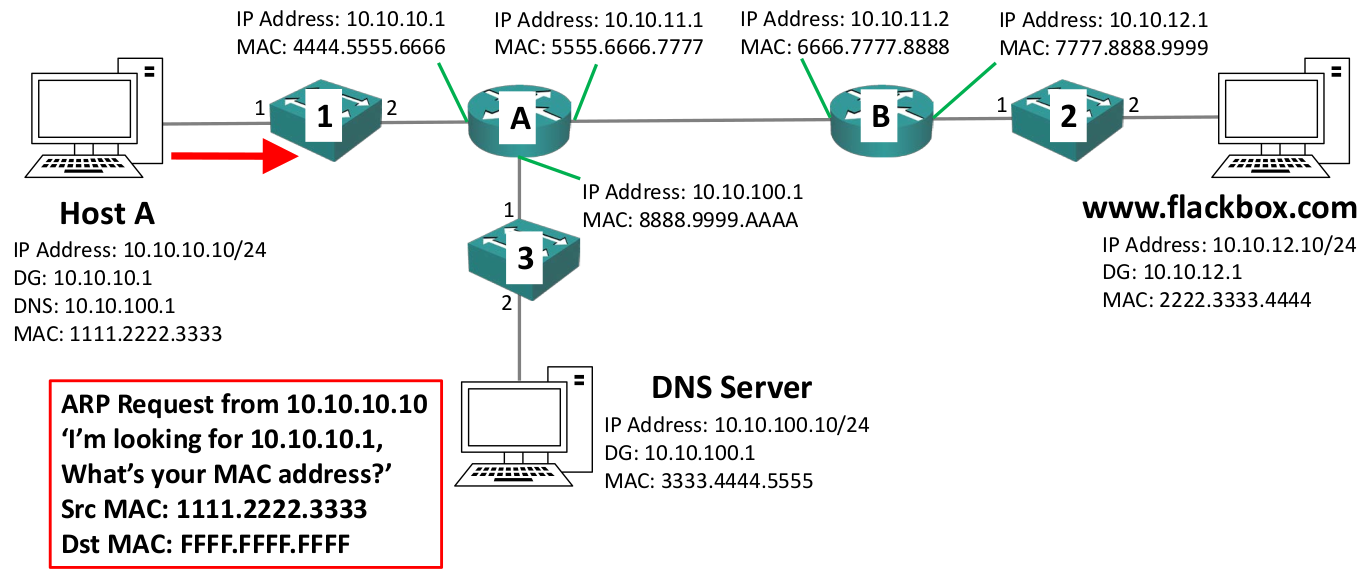
\includegraphics[width=\linewidth]{img/img17}
	\end{center}
\end{frame}

\begin{frame}{The Life of a Packet}
	\begin{itemize}
		\item The ARP request will be received by Switch 1
		\item Switch 1 will add an entry in its MAC address table mapping Host A’s MAC address 1111.2222.3333 to Port 1
		\item Switch 1 will flood the broadcast traffic out all ports apart from the one it was received on
	\end{itemize}
\end{frame}

\begin{frame}{The Life of a Packet}
	\begin{center}
		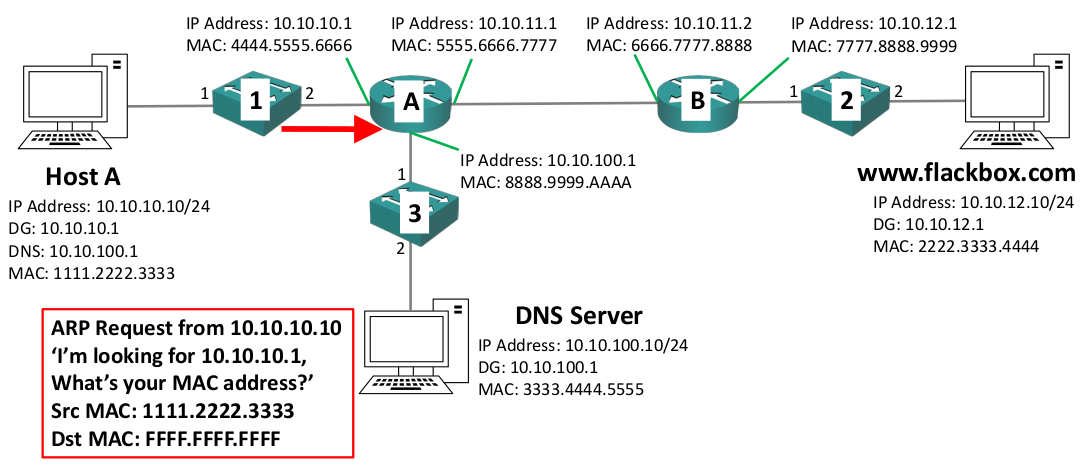
\includegraphics[width=\linewidth]{img/img18}
	\end{center}
\end{frame}

\begin{frame}{The Life of a Packet}
	\begin{itemize}
		\item The ARP request will hit Router A’s interface 10.10.10.1
		\item Router A will process the ARP request and see it is for itself
		\item Router A will send a unicast ARP reply to Host A
		\item Router A will add an entry for Host A mapping IP address 10.10.10.10 to MAC address 1111.2222.3333 to its ARP cache
	\end{itemize}
\end{frame}

\begin{frame}{The Life of a Packet}
	\begin{center}
		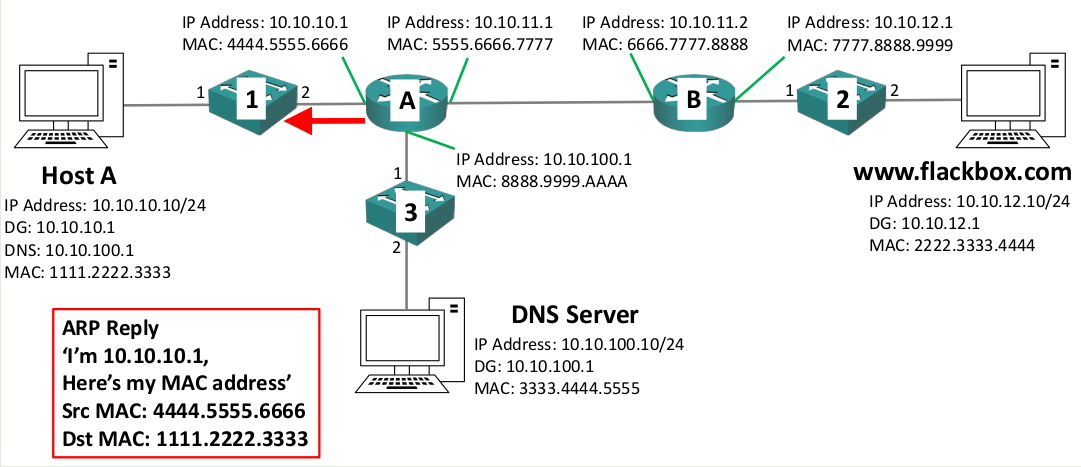
\includegraphics[width=\linewidth]{img/img19}
	\end{center}
\end{frame}

\begin{frame}{The Life of a Packet}
	\begin{itemize}
		\item Switch 1 will add an entry in its MAC address table mapping Router A’s MAC address 4444.5555.6666 to Port 2
		\item Switch 1 will send the ARP reply out only Port 1 which Host A is plugged into (which it already has in its MAC address table)
	\end{itemize}
\end{frame}

\begin{frame}{The Life of a Packet}
	\begin{center}
		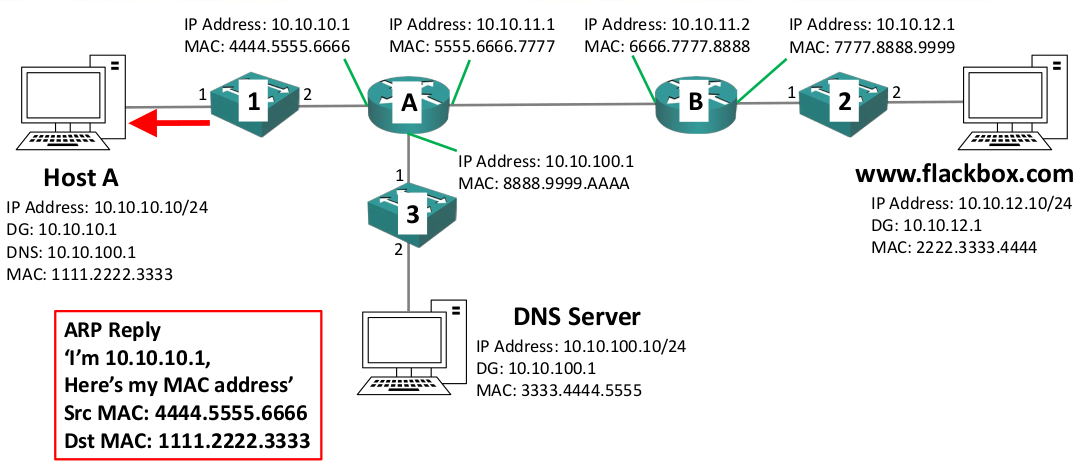
\includegraphics[width=\linewidth]{img/img20}
	\end{center}
\end{frame}

\begin{frame}{The Life of a Packet}
	\begin{itemize}
		\item Host A will add an entry for Router A mapping IP address 10.10.10.1 to MAC address 4444.5555.6666 to its ARP cache
		\item It will use this whenever it needs to send traffic to another IP subnet
		\item Host A will send the DNS request for www.flackbox.com
	\end{itemize}
\end{frame}

\begin{frame}{The Life of a Packet}
	\begin{center}
		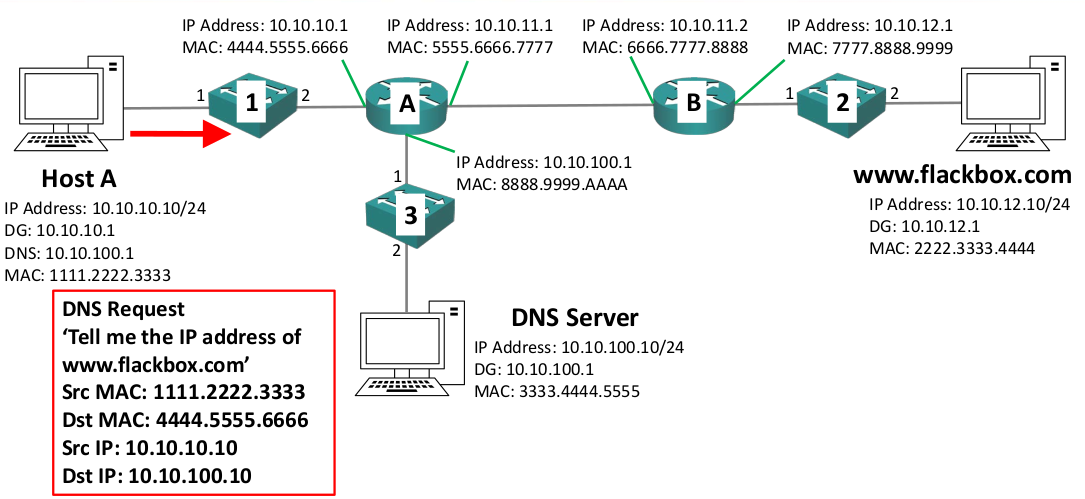
\includegraphics[width=\linewidth]{img/img21}
	\end{center}
\end{frame}

\end{document}
